\documentclass[11pt, oneside]{article}   	% use "amsart" instead of "article" for AMSLaTeX format
\usepackage{geometry}                		% See geometry.pdf to learn the layout options. There are lots.
\geometry{letterpaper}                   		% ... or a4paper or a5paper or ... 
%\geometry{landscape}                		% Activate for rotated page geometry
%\usepackage[parfill]{parskip}    		% Activate to begin paragraphs with an empty line rather than an indent
\usepackage{graphicx}				% Use pdf, png, jpg, or eps§ with pdflatex; use eps in DVI mode
								% TeX will automatically convert eps --> pdf in pdflatex
\usepackage{amssymb}
\usepackage{amsmath}
\usepackage{algorithm}% http://ctan.org/pkg/algorithm
\usepackage{algpseudocode}% http://ctan.org/pkg/algorithmicx
\usepackage{mathtools,xparse}
\usepackage{dsfont}
%SetFonts

%SetFonts


\title{CSE512 HW4}
\author{Tim Zhang (110746199)}
\date{}							% Activate to display a given date or no date

\begin{document}
\maketitle
%\section{}
%\subsection{}

\DeclarePairedDelimiter{\norm}{\lVert}{\rVert}

\section{SGD for Multiclass Classification with Kernels and Costs}
\subsection{Question 2: Updates}
\subsubsection{(a)}
 \[
   \Delta =
  \left[ {\begin{array}{cccccccccc}
   0 & 1 & 1 & 1 & 1 & 1 & 1 & 1 & 1  & 1\\
   1 & 0 & 1 & 1 & 1 & 1 & 1 & 1 & 1  & 1\\
   1 & 1 & 0 & 1 & 1 & 1 & 1 & 1 & 1 & 1\\
   1 & 1 & 1 & 0 & 1 & 1 & 1 & 1 & 1 & 1\\
   1 & 1 & 1 & 1 & 0 & 1 & 1 & 1 & 1 & 1\\
   1 & 1 & 1 & 1 & 1 & 0 & 1 & 1 & 1 & 1\\
   1 & 1 & 1 & 1 & 1 & 1 & 0 & 1 & 1 & 1\\
   1 & 1 & 1 & 1 & 1 & 1 & 1 & 0 & 1 & 1\\
   1 & 1 & 1 & 1 & 1 & 1 & 1 & 1 & 0 & 1\\
   1 & 1 & 1 & 1 & 1 & 1 & 1 & 1 & 1 & 0\\
  \end{array} } \right]
\]

\subsubsection{(b)}
 \[
   \Delta =
  \left[ {\begin{array}{cccccccccc}
   0 & 1 & 2 & 2 & 2 & 2 & 2 & 2 & 2 & 2\\
   1 & 0 & 1 & 2 & 2 & 2 & 2 & 2 & 2 & 2\\
   2 & 1 & 0 & 1 & 2 & 2 & 2 & 2 & 2 & 2\\
   2 & 2 & 1 & 0 & 1 & 2 & 2 & 2 & 2 & 2\\
   2 & 2 & 2 & 1 & 0 & 1 & 2 & 2 & 2 & 2\\
   2 & 2 & 2 & 2 & 1 & 0 & 1 & 2 & 2 & 2\\
   2 & 2 & 2 & 2 & 2 & 1 & 0 & 1 & 2 & 2\\
   2 & 2 & 2 & 2 & 2 & 2 & 1 & 0 & 1 & 2\\
   2 & 2 & 2 & 2 & 2 & 2 & 2 & 1 & 0 & 1\\
   2 & 2 & 2 & 2 & 2 & 2 & 2 & 2 & 1 & 0\\
  \end{array} } \right]
\]

\newpage{}
\subsubsection{(c)}
Fix $\hat{y} \in \max_{y' \in \{1, \ldots, k\}} \Delta(y', y_t) + \langle \boldsymbol{w}_{t, y'}, \phi(\boldsymbol{x}_t) \rangle - \langle \boldsymbol{w}_{t, y_t}, \phi(\boldsymbol{x}_t) \rangle$.  

Then:
\begin{gather*}
\nabla_{\boldsymbol{w}_{t, i}}\ell(\boldsymbol{w}_{t, i}, \phi(\boldsymbol{x}_t), y_t) = \\
\nabla_{\boldsymbol{w}_{t, i}} \Delta(\hat{y}, y_t) + \langle \boldsymbol{w}_{t, \hat{y}}, \phi(\boldsymbol{x}_t) \rangle - \langle \boldsymbol{w}_{t, y_t}, \phi(\boldsymbol{x}_t) \rangle =
\begin{cases} 
0 &\quad\text{ if $\hat{y} = y_t = i \lor \hat{y} \neq i$ and $y_t \neq i$ }\\
\phi(\boldsymbol{x}_t) &\quad\text{ if $\hat{y} = i$ and $y_t \neq i$}\\
-\phi(\boldsymbol{x}_t) &\quad\text{ if $\hat{y} \neq i$ and $y_t = i$}
\end{cases}
\end{gather*}
Assuming that $\Delta(y, y')$ is not a function of $\boldsymbol{w}_t$ $\blacksquare$

\subsection{Question 3: SGD with kernels}
\subsubsection{(a)}
Let $\alpha_{j, i}$ be constructed using the fixed $\hat{y}$ discussed above.

Then:
\begin{gather*}
\alpha_{j, i} =
\begin{cases} 
0 &\quad\text{ if $\hat{y} = y_j = i \lor \hat{y} \neq i$ and $y_j \neq i$ }\\
-\eta_j &\quad\text{ if $\hat{y} = i$ and $y_j \neq i$}\\
\eta_j &\quad\text{ if $\hat{y} \neq i$ and $y_j = i$}
\end{cases}
\end{gather*}

This clearly shows that $\boldsymbol{w}_{t, i} = \sum_{j = 1}^{t-1}\alpha_{j, i}\phi(\boldsymbol{x}_j)$ by observing the definition of $\alpha_{j, i}$ and of $\nabla_{\boldsymbol{w}_{j, i}}\ell(\boldsymbol{w}_{j, i}, \phi(\boldsymbol{x}_j), y_j)$.  Under the assumption that each weight vector is initialized to $\boldsymbol{0}$.

Note that the signs are flipped in the definition of $\alpha_{j, i}$ as compared to the subgradient given that the SGD update rule is $\boldsymbol{w}_{t + 1, i} = \boldsymbol{w}_{t, i} - \eta_t \boldsymbol{g}_{t, i}$.

Giving a formal inductive proof (and starting from $t = 0$) the basis case is:
\begin{gather*}
\boldsymbol{w}_{1, i} = \boldsymbol{w}_{0, i} - \eta_1 \boldsymbol{g}_{1, i} = \boldsymbol{0} - \eta_1 \boldsymbol{g}_{1, i} = \boldsymbol{0} + \alpha_{1, i}\phi(\boldsymbol{x}_1)
\end{gather*}
Using the inductive hypothesis that $\boldsymbol{w}_{t, i} = \sum_{j = 1}^{t-1}\alpha_{j, i}\phi(\boldsymbol{x}_j)$:
\begin{gather*}
\boldsymbol{w}_{t + 1} = \boldsymbol{w}_{t, i} - \eta_{t} \boldsymbol{g}_{t, i} \\
=  - \eta_{t} \boldsymbol{g}_{t, i} + \sum_{j = 1}^{t-1}\alpha_{j, i}\phi(\boldsymbol{x}_j)\\
=  \alpha_{t, i}\phi(\boldsymbol{x}_t) + \sum_{j = 1}^{t-1}\alpha_{j, i}\phi(\boldsymbol{x}_j)\\
=  \sum_{j = 1}^{t}\alpha_{j, i}\phi(\boldsymbol{x}_j) \text{ } \blacksquare
\end{gather*}

\newpage{}
\subsubsection{(b)}
\begin{gather*}
\langle \boldsymbol{w}_{t, i}, \phi(\boldsymbol{x}_t) \rangle = \langle \sum_{j = 1}^{t-1}\alpha_{j, i}\phi(\boldsymbol{x}_j), \phi(\boldsymbol{x}_t) \rangle\\
= \sum_{j = 1}^{t-1} \langle \alpha_{j, i}\phi(\boldsymbol{x}_j), \phi(\boldsymbol{x}_t) \rangle\\
= \sum_{j = 1}^{t-1} \alpha_{j, i} \langle \phi(\boldsymbol{x}_j), \phi(\boldsymbol{x}_t) \rangle\\
= \sum_{j = 1}^{t-1} \alpha_{j, i} k(\boldsymbol{x}_j, \boldsymbol{x}_t)
\end{gather*}
Where the second line is from distributivity of dot product, the third line is because $\alpha_{j, i}$ is a scalar, and the last line the the definition of $k(\boldsymbol{x}, \boldsymbol{x'})$ $\blacksquare$
\newpage{}
\subsection{Question 4: Implementation and Use}
\subsubsection{(a)}
\textbf{NOTE:} It is assumed that $X \in \mathbb{R}^{m \times d}$ and $y \in \mathbb{R}^{m \times 1}$.
\begin{verbatim}
%
% Function computes kernel SGD
%
function [alpha, Xsv] = train_mhinge_krnel_sgd(Xtr, ytr, Delta, p)
    [m, d] = size(Xtr);     % Dimensions of data
    k = 10;                 % Number of classes
    alpha = zeros(1, k);    % Matrix of alphas
    Xsv = zeros(1, d);      % Saved samples
    
    % Bootstrap the first example
    max = 0;
    yhat = 0;
    
    % Find yhat
    for i = 1: k
        loss = Delta(i, ytr(1));
        
        if loss > max
            max = loss;
            yhat = i;
        end
    end
    
    Xsv(1, :) = Xtr(1, :);  % Initialize Xsv to only the first example
    
    % Compute alpha_{j, i} where eta_1 = 1
    for i = 1: k
        if i == ytr(1) + 1
            alpha(1, i) = 1;
        elseif i == yhat
            alpha(1, i) = -1;
        else
            alpha(1, i) = 0;
        end
    end
    
    % Compute SGD over remaining training examples
    for t = 2: m
        y = ytr(t) + 1;  % Label for current training sample
        x = Xtr(t, :);   % Current sample
        cur_alpha = zeros(1, k);  % Current alpha
        eta = 1/sqrt(t);  % Learning rate
        
        % Determine yhat
        yhat = maximize_loss(alpha, Xsv, Delta, k, x, y, p);
        
        % Update Alpha
        for i = 1: k
            if i ~= yhat && i == y
                cur_alpha(1, i) = eta;
            
            elseif i == yhat && i ~= y
                cur_alpha(1, i) = -1 * eta;
            
            % Otherwise either y = yhat = i or y ~= i and yhat ~= i
            else 
                cur_alpha(1, i) = 0;
            end
        end
        
        % If an update occured
        if any(cur_alpha)
            alpha = [alpha; cur_alpha];
            Xsv = [Xsv; x];
        end
    end
end










%
% Function computes loss at timestep
%
function loss = compute_loss(alpha, y, ker)
    loss = 0;   % Initial loss
    [t, ~] = size(alpha);
    
    for i = 1: t
        loss = loss + (alpha(i, y) * ker(i));
    end
end

%
% Function returns class which maximizes loss
%
function yhat = maximize_loss(alpha, Xsv, Delta, k, x, y, p)
    max = intmin;  % Maximum loss value
    yhat = 0;      % Maximum loss label
    
    % Precompute the kernel function
    ker = kernel(x, Xsv, p);
    
    % Compute loss term involving y_t
    y_loss = compute_loss(alpha, y, ker);
    
    % Find y' which maximizes loss
    for i = 1: k
        if i == y
            loss = Delta(i, y);
        else
            yhat_loss = compute_loss(alpha, i, ker);
            loss = Delta(i, y) + yhat_loss - y_loss;
        end

        % Update maximizer
        if loss > max
            max = loss;
            yhat = i;
        end
    end
end

%
% Function computes polynomial kernel
%
function ker = kernel(x, Xsv, p)
    [m, ~] = size(Xsv);
    ker = zeros(m, 1);
    
    for i = 1: m
        ker(i) = (x * Xsv(i, :)')^p;
    end
end
\end{verbatim}

\newpage{}
\subsubsection{(b)}
\begin{verbatim}
%
% Function computes the predicted classes
%
function [ypred] = test_mhinge_kernel_sgd(alpha, Xsv, Xte, p)
    [m, d] = size(Xte);
    [t, k] = size(alpha);
    ypred = zeros(m, 1);
    disp(m);
    
    % Predict for each test example
    for i = 1: m
        max = intmin;  % Determine most likely class
        pred = 0;
        
        % Precompute the kernel function
        ker = kernel(Xte(i, :), Xsv, p);
        
        % Calculate scores for each class predictor
        for class = 1: k
            score = 0;
            
            % Compute <w, x>
            for j = 1: t
                score = score + (alpha(j, class) * ker(j));
            end

            % Update prediction
            if score > max
                max = score;
                pred = class;
            end
        end
        
        ypred(i) = pred - 1;  % Classes range from 0-9, k from 1-10
    end
end
\end{verbatim}

\newpage{}
\subsubsection{(c)}
In the following confusion matrices the rows are the correct class and the columns are the predicted labels.\\\\
\textbf{Cost Matrix $\Delta_{2.a}$} \\\\
Test error $= \verb!0.0345!$
 \[
  \text{Confusion matrix} =
  \left[ {\begin{array}{ccccccccccc}
   & \underline{\textbf{0}} & \underline{\textbf{1}} & \underline{\textbf{2}} & \underline{\textbf{3}} & \underline{\textbf{4}} & \underline{\textbf{5}} & \underline{\textbf{6}} & \underline{\textbf{7}} & \underline{\textbf{8}} & \underline{\textbf{9}}\\
   \underline{\textbf{0}} & \textbf{963} & 1 & 2 & 1 & 0 & 2 & 9 & 1 & 1 & 0\\
   \underline{\textbf{1}} & 0 & \textbf{1125} & 2 & 1 & 0 & 1 & 1 & 0 & 5 & 0\\
   \underline{\textbf{2}} & 5 & 2 & \textbf{995} & 6 & 4 & 0 & 5 & 6 & 9 & 0\\
   \underline{\textbf{3}} & 1 & 0 & 1 & \textbf{980} & 0 & 8 & 1 & 3 & 11 & 5\\
   \underline{\textbf{4}} & 2 & 1 & 3 & 0 & \textbf{951} & 0 & 5 & 1 & 3 & 16\\
   \underline{\textbf{5}} & 3 & 0 & 1 & 10 & 2 & \textbf{853} & 12 & 1 & 8 & 2\\
   \underline{\textbf{6}} & 11 & 3 & 2 & 0 & 8 & 5 & \textbf{925} & 0 & 4 & 0\\
   \underline{\textbf{7}} & 3 & 6 & 6 & 4 & 3 & 1 & 0 & \textbf{989} & 1 & 15\\
   \underline{\textbf{8}} & 5 & 1 & 1 & 10 & 3 & 1 & 6 & 7 & \textbf{936} & 4\\
   \underline{\textbf{9}} & 6 & 7 & 2 & 9 & 29 & 4 & 4 & 6 & 4 & \textbf{938}\\
  \end{array} } \right]
\]
\textbf{Cost Matrix $\Delta_{2.b}$}\\\\
Test error $= \verb!0.0345!$
 \[
  \text{Confusion matrix} =
  \left[ {\begin{array}{ccccccccccc}
   & \underline{\textbf{0}} & \underline{\textbf{1}} & \underline{\textbf{2}} & \underline{\textbf{3}} & \underline{\textbf{4}} & \underline{\textbf{5}} & \underline{\textbf{6}} & \underline{\textbf{7}} & \underline{\textbf{8}} & \underline{\textbf{9}}\\
   \underline{\textbf{0}} & \textbf{963} & 1 & 2 & 1 & 0 & 2 & 9 & 1 & 1 & 0\\
   \underline{\textbf{1}} & 0 & \textbf{1125} & 2 & 1 & 0 & 1 & 1 & 0 & 5 & 0\\
   \underline{\textbf{2}} & 5 & 2 & \textbf{995} & 6 & 4 & 0 & 5 & 6 & 9 & 0\\
   \underline{\textbf{3}} & 1 & 0 & 1 & \textbf{980} & 0 & 8 & 1 & 3 & 11 & 5\\
   \underline{\textbf{4}} & 2 & 1 & 3 & 0 & \textbf{951} & 0 & 5 & 1 & 3 & 16\\
   \underline{\textbf{5}} & 3 & 0 & 1 & 10 & 2 & \textbf{853} & 12 & 1 & 8 & 2\\
   \underline{\textbf{6}} & 11 & 3 & 2 & 0 & 8 & 5 & \textbf{925} & 0 & 4 & 0\\
   \underline{\textbf{7}} & 3 & 6 & 6 & 4 & 3 & 1 & 0 & \textbf{989} & 1 & 15\\
   \underline{\textbf{8}} & 5 & 1 & 1 & 10 & 3 & 1 & 6 & 7 & \textbf{936} & 4\\
   \underline{\textbf{9}} & 6 & 7 & 2 & 9 & 29 & 4 & 4 & 6 & 4 & \textbf{938}\\
  \end{array} } \right]
\]

\newpage{}
\begin{verbatim}
%
% Function ouputs the accuracy of the prediction
%
function [correct, misclassified] = test_prediction(ypred, yte)
    [m, ~] = size(yte);
    correct = zeros(10, 1);         % Correct predictions per class
    misclassified = zeros(10, 10);  % (correct class, prediction)
    
    for i = 1: m
        % If the prediction was wrong store prediction
        if ypred(i) ~= yte(i)
            misclassified(yte(i) + 1, ypred(i) + 1) = 
            misclassified(yte(i) + 1, ypred(i) + 1) + 1;
        else
            correct(ypred(i) + 1) = correct(ypred(i) + 1) + 1;
        end
    end
    
    disp('Accuracy:');
    disp(sum(correct)/m);
end
\end{verbatim}
\newpage{}
\section{Question 5: Boosting}
Let $Z = \sum_{i = 1}^{m} D_t(\boldsymbol{x}_i, y_i) \cdot \text{exp}(-w_t y_i f_t(\boldsymbol{x_i}))$ and $\epsilon_t = \sum_{i : y_i \neq f_t(\boldsymbol{x}_i)}D_t(\boldsymbol{x}_i, y_i)$:
\begin{gather*}
\sum_{i = 1}^{m}D_{t + 1}(\boldsymbol{x}_i, y_i) \cdot \mathds{1}[y_i \neq f_t(\boldsymbol{x_i})] = \sum_{i : y_i \neq f_t(\boldsymbol{x}_i)}D_{t + 1}(\boldsymbol{x}_i, y_i) \\
= \frac{1}{Z} \sum_{i : y_i \neq f_t(\boldsymbol{x}_i)}D_{t}(\boldsymbol{x}_i, y_i) \cdot \text{exp}(w_t)\\
= \frac{\text{exp}(w_t) \epsilon_t}{Z}
\end{gather*}
Rewriting $Z$:
\begin{gather*}
Z = \sum_{i = 1}^{m} D_t(\boldsymbol{x}_i, y_i) \cdot \text{exp}(-w_t y_i f_t(\boldsymbol{x_i}))\\
= \text{exp}(w_t) \sum_{i : y_i \neq f_t(\boldsymbol{x}_i)}D_t(\boldsymbol{x}_i, y_i) + \text{exp}(-w_t) \sum_{i : y_i = f_t(\boldsymbol{x}_i)}D_t(\boldsymbol{x}_i, y_i)\\
= \text{exp}(w_t) \epsilon_t + \text{exp}(-w_t) \sum_{i : y_i = f_t(\boldsymbol{x}_i)}D_t(\boldsymbol{x}_i, y_i)
\end{gather*}
Then:
\begin{gather*}
\sum_{i = 1}^{m}D_{t + 1}(\boldsymbol{x}_i, y_i) \cdot \mathds{1}[y_i \neq f_t(\boldsymbol{x_i})] = \frac{\text{exp}(w_t) \epsilon_t}{\text{exp}(w_t) \epsilon_t + \text{exp}(-w_t) \sum_{i : y_i = f_t(\boldsymbol{x}_i)}D_t(\boldsymbol{x}_i, y_i)}\\
= \frac{1}{(\text{exp}(w_t) \epsilon_t)^{-1} \cdot \text{exp}(w_t) \epsilon_t + (\text{exp}(w_t) \epsilon_t)^{-1} \cdot \text{exp}(-w_t) \sum_{i : y_i = f_t(\boldsymbol{x}_i)}D_t(\boldsymbol{x}_i, y_i)}\\
= \frac{1}{1 + (\text{exp}(w_t) \epsilon_t)^{-1} \cdot \text{exp}(-w_t) \sum_{i : y_i = f_t(\boldsymbol{x}_i)}D_t(\boldsymbol{x}_i, y_i)}
\end{gather*}
It remains to show that $(\text{exp}(w_t) \epsilon_t)^{-1} \cdot \text{exp}(-w_t) \sum_{i : y_i = f_t(\boldsymbol{x}_i)}D_t(\boldsymbol{x}_i, y_i) = 1$:
\begin{gather*}
(\text{exp}(w_t) \epsilon_t)^{-1} \cdot \text{exp}(-w_t) \sum_{i : y_i = f_t(\boldsymbol{x}_i)}D_t(\boldsymbol{x}_i, y_i) = \frac{\text{exp}(-w_t) \sum_{i : y_i = f_t(\boldsymbol{x}_i)}D_t(\boldsymbol{x}_i, y_i)}{\text{exp}(w_t) \epsilon_t}\\
= \frac{(\frac{1}{\epsilon_t} - 1)^{-1/2}\sum_{i : y_i = f_t(\boldsymbol{x}_i)}D_t(\boldsymbol{x}_i, y_i)}{(\frac{1}{\epsilon_t} - 1)^{1/2}\epsilon_t}\\
= \frac{\sum_{i : y_i = f_t(\boldsymbol{x}_i)}D_t(\boldsymbol{x}_i, y_i)}{(\frac{1}{\epsilon_t} - 1)^{1/2}(\frac{1}{\epsilon_t} - 1)^{1/2}\epsilon_t}\\
= \frac{\sum_{i : y_i = f_t(\boldsymbol{x}_i)}D_t(\boldsymbol{x}_i, y_i)}{(\frac{1}{\epsilon_t} - 1)\epsilon_t}\\
= \frac{\sum_{i : y_i = f_t(\boldsymbol{x}_i)}D_t(\boldsymbol{x}_i, y_i)}{1 - \epsilon_t}\\
= \frac{\sum_{i : y_i = f_t(\boldsymbol{x}_i)}D_t(\boldsymbol{x}_i, y_i)}{\sum_{i : y_i = f_t(\boldsymbol{x}_i)}D_t(\boldsymbol{x}_i, y_i)} = 1\\
\end{gather*}
Where the last line follows from the fact that $D_t$ is a probability distribution and thus $1 - \epsilon_t = 1 - \sum_{i : y_i \neq f_t(\boldsymbol{x}_i)}D_t(\boldsymbol{x}_i, y_i) = \sum_{i : y_i = f_t(\boldsymbol{x}_i)}D_t(\boldsymbol{x}_i, y_i)$ $\blacksquare$
\newpage{}
\section{PCA via Successive Deflation}
\subsection{Question 6}
\subsubsection{(a)}
By definition $\boldsymbol{\tilde{C}} = \frac{1}{m} \boldsymbol{\tilde{X}} \boldsymbol{\tilde{X}}^{\top}$ then solving for $\boldsymbol{\tilde{X}} \boldsymbol{\tilde{X}}^{\top}$:
\begin{gather*}
\boldsymbol{\tilde{X}} \boldsymbol{\tilde{X}}^{\top}
= (\boldsymbol{I} - \boldsymbol{v}_{1} \boldsymbol{v}_{1}^{\top})\boldsymbol{X} ((\boldsymbol{I} - \boldsymbol{v}_{1} \boldsymbol{v}_{1}^{\top})\boldsymbol{X})^{\top}\\
= (\boldsymbol{I} - \boldsymbol{v}_{1} \boldsymbol{v}_{1}^{\top})\boldsymbol{X} \boldsymbol{X}^{\top}(\boldsymbol{I} - \boldsymbol{v}_{1} \boldsymbol{v}_{1}^{\top}) \\
= (\boldsymbol{I} - \boldsymbol{v}_{1} \boldsymbol{v}_{1}^{\top})(\boldsymbol{X} \boldsymbol{X}^{\top} - \boldsymbol{X} \boldsymbol{X}^{\top}\boldsymbol{v}_{1} \boldsymbol{v}_{1}^{\top})\\
= (\boldsymbol{I} - \boldsymbol{v}_{1} \boldsymbol{v}_{1}^{\top})(\boldsymbol{X} \boldsymbol{X}^{\top} - m\lambda_1\boldsymbol{v}_{1} \boldsymbol{v}_{1}^{\top})\\
= \boldsymbol{X} \boldsymbol{X}^{\top} - m\lambda_1\boldsymbol{v}_{1} \boldsymbol{v}_{1}^{\top} - \boldsymbol{v}_{1} \boldsymbol{v}_{1}^{\top}\boldsymbol{X} \boldsymbol{X}^{\top} + \boldsymbol{v}_{1} \boldsymbol{v}_{1}^{\top}m\lambda_1\boldsymbol{v}_{1} \boldsymbol{v}_{1}^{\top}\\
= \boldsymbol{X} \boldsymbol{X}^{\top} - m\lambda_1\boldsymbol{v}_{1} \boldsymbol{v}_{1}^{\top} - \boldsymbol{v}_{1} \boldsymbol{v}_{1}^{\top}\boldsymbol{X} \boldsymbol{X}^{\top} + m\lambda_1\boldsymbol{v}_{1} \boldsymbol{v}_{1}^{\top}\boldsymbol{v}_{1} \boldsymbol{v}_{1}^{\top}\\
= \boldsymbol{X} \boldsymbol{X}^{\top} - m\lambda_1\boldsymbol{v}_{1} \boldsymbol{v}_{1}^{\top} - \boldsymbol{v}_{1} \boldsymbol{v}_{1}^{\top}\boldsymbol{X} \boldsymbol{X}^{\top} + m\lambda_1\boldsymbol{v}_{1} \boldsymbol{v}_{1}^{\top}\\
= \boldsymbol{X} \boldsymbol{X}^{\top} - \boldsymbol{v}_{1} \boldsymbol{v}_{1}^{\top}\boldsymbol{X} \boldsymbol{X}^{\top}\\
= (\boldsymbol{I} - \boldsymbol{v}_{1} \boldsymbol{v}_{1}^{\top})\boldsymbol{X} \boldsymbol{X}^{\top}\\
= (((\boldsymbol{I} - \boldsymbol{v}_{1} \boldsymbol{v}_{1}^{\top})\boldsymbol{X} \boldsymbol{X}^{\top})^{\top})^{\top}\\
= ((\boldsymbol{X} \boldsymbol{X}^{\top})^{\top}(\boldsymbol{I} - \boldsymbol{v}_{1} \boldsymbol{v}_{1}^{\top})^{\top})^{\top}\\
= (\boldsymbol{X} \boldsymbol{X}^{\top}(\boldsymbol{I} - \boldsymbol{v}_{1} \boldsymbol{v}_{1}^{\top}))^{\top}\\
= (\boldsymbol{X} \boldsymbol{X}^{\top} - \boldsymbol{X} \boldsymbol{X}^{\top}\boldsymbol{v}_{1} \boldsymbol{v}_{1}^{\top})^{\top}\\
= (\boldsymbol{X} \boldsymbol{X}^{\top} - m\lambda_1\boldsymbol{v}_{1} \boldsymbol{v}_{1}^{\top})^{\top}\\
= (\boldsymbol{X} \boldsymbol{X}^{\top})^{\top} - (m\lambda_1\boldsymbol{v}_{1} \boldsymbol{v}_{1}^{\top})^{\top}\\
= \boldsymbol{X} \boldsymbol{X}^{\top} - m\lambda_1\boldsymbol{v}_{1} \boldsymbol{v}_{1}^{\top}\\
\end{gather*}

Thus $\boldsymbol{\tilde{C}} = \frac{1}{m} \boldsymbol{\tilde{X}} \boldsymbol{\tilde{X}}^{\top} = \frac{1}{m} \boldsymbol{X} \boldsymbol{X}^{\top} - \lambda_1\boldsymbol{v}_{1} \boldsymbol{v}_{1}^{\top}$ $\blacksquare$

\subsubsection{(b)}
First note that $\boldsymbol{\tilde{C}} = \frac{1}{m} \boldsymbol{X} \boldsymbol{X}^{\top} - \lambda_1\boldsymbol{v}_{1} \boldsymbol{v}_{1}^{\top} = \boldsymbol{C} - \lambda_1\boldsymbol{v}_{1} \boldsymbol{v}_{1}^{\top}$:
\begin{gather*}
\boldsymbol{\tilde{C}}\boldsymbol{v}_j = (\boldsymbol{C} - \lambda_1\boldsymbol{v}_{1} \boldsymbol{v}_{1}^{\top})\boldsymbol{v}_j \\
= \boldsymbol{C}\boldsymbol{v}_j - \lambda_1\boldsymbol{v}_{1} \boldsymbol{v}_{1}^{\top}\boldsymbol{v}_j\\
= \lambda_j\boldsymbol{v}_j
\end{gather*}
Where the last equality is due to the definition of $\lambda_j\boldsymbol{v}_j$ and the fact that $\boldsymbol{v}_{1}^{\top}\boldsymbol{v}_j = 0$ for $j \neq 1$ $\blacksquare$

\subsubsection{(c)}
It suffices to show that $\lambda_1$, $\boldsymbol{v}_1$ are no longer the largest eigenvalue/eigenvector pair of $\boldsymbol{\tilde{C}}$:
\begin{gather*}
\boldsymbol{\tilde{C}}\boldsymbol{v}_1 = (\boldsymbol{C} - \lambda_1\boldsymbol{v}_{1} \boldsymbol{v}_{1}^{\top})\boldsymbol{v}_1 \\
= \boldsymbol{C}\boldsymbol{v}_1 - \lambda_1\boldsymbol{v}_{1} \boldsymbol{v}_{1}^{\top}\boldsymbol{v}_1\\
= \lambda_1\boldsymbol{v}_1 - \lambda_1\boldsymbol{v}_1\\
= 0 = \lambda_1'\boldsymbol{v}_1
\end{gather*}
Thus $\lambda_1' = 0$ and is now strictly smaller than $\lambda_2$ (since $\boldsymbol{v}_i \neq 0$ by definition) thus $\boldsymbol{u} = \boldsymbol{v}_2$ since the eigenvectors are sorted by eigenvalue $\blacksquare$

\subsubsection{(d)}
\begin{verbatim}
function [lambdas, vectors] = compute_k_eigenvectors(C, k, f):
    lambdas = zeros(k, 1);  % Vector of eigenvalues
    U = zeros(k, 1);  % Vector of eigenvectors
    
    for i = 1: k
        [lambda, u] = f(C);  % Call oracle function
        lambdas(i) = lambda;
        U(i) = u;
        
        C = C - (lambda * u * u');  % Compute deflated covariance
    end
end
\end{verbatim}
\newpage{}
\section{ Clustering with $k$-means}
\subsection{Question 7}
\subsubsection{(a)}
\begin{verbatim}
%
% Function computes the set of k centers via k-means clustering
%
function M = kmeans(X, k, T)
    [m, d] = size(X);   % Dimensions of data
    M = zeros(k, d);    % Matrix of k centers
    C = zeros(m, 1);    % Entries are {1, ..., k} for sample cluster
    
    % Sequentially assign centers as first k examples
    for i = 1: k
        M(i, :) = X(i, :);
    end
    
    % Iterate a max of T times
    for i = 1: T
        converged = true;  % Tracks if algorithm has converged
        
        % Assign each sample to nearest center
        for j = 1: m
            prev = C(j);  % Track previous center
            C(j) = compute_nearest_center(M, X(j, :), k);
            
            if C(j) ~= prev
                converged = false;
            end
        end
        
        % Terminate on convergence
        if converged
            break;
        end
        
        % Recompute centers
        compute_centers(M, C, X);    
    end
end

%
% Function returns the index of the closest center to sample
%
function c = compute_nearest_center(M, x, k)
    c = 0;             % Index of nearest center
    closest = intmax;  % Current value closest distance
    
    for i = 1: k
        dist = norm(x - M(i, :));  % Compute distance via l2 norm
        
        if dist < closest
            c = i;
            closest = dist;
        end
    end
end

%
% Function recomputes centers as average vector of cluster
%
function compute_centers(M, C, X)
    [k, d] = size(M);
    [m, ~] = size(X);
    
    % Recompute center for each cluster
    for i = 1: k
        center = zeros(1, d);  % Average vector
        m_cluster = 0;         % Number of samples in cluster
        
        for j = 1: m
            if C(j) == i
                center = center + X(i, :);
                m_cluster = m_cluster + 1;
            end
        end
        
        M(i, :) = center ./ m_cluster;
    end
end
\end{verbatim}

\subsubsection{(b)}
\begin{verbatim}
%
% Function plots iterations of k-means via metric
%
function plot(X, y, k_max, T, metric)
    k = 2;
    val = [];  % Holds each iterations value
    
    while k <= k_max
        M = kmeans(X, k, T);  % Compute centers
        
        if strcmp(metric, 'Sum of Squares')
            val = [val sum_of_squares(M, X, k)]; 
        elseif strcmp(metric, 'Purity')
            val = [val, purity(M, X, y, k)];
        else
            disp('Invalid metric');
            return
        end
        
        k = k + 2;  % Iterate by 2
    end
    
    % Plot values
    plot(val);
end

%
% Function computes sum of squares
%
function sum = sum_of_squares(M, X, k)
    [m, ~] = size(X);
    C = zeros(m, 1);  % Entries are {1, ..., k} for sample cluster
    sum = 0;
    
    % Assign each sample to nearest center
    for i = 1: m
        C(i) = compute_nearest_center(M, X(i, :), k);
    end
    
    % Calculate squared distance for each cluster
    for i = 1: m
        sum = sum + norm(X(i, :) - M(C(i), :))^2;
    end
end
\end{verbatim}
\begin{figure}[h!]
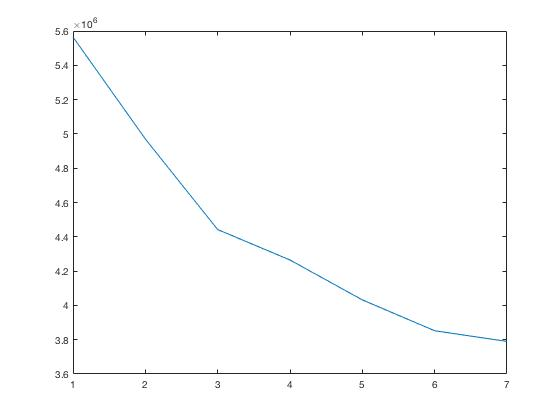
\includegraphics[width=\textwidth]{sum_of_squares.jpg}
\end{figure}
Horizontal axis represents the $ith$ iteration, for example $3$ is the iteration where $k = 6$.
\newpage{}
\subsubsection{(c)}
\begin{verbatim}
%
% Function computes purity
%
function purity = purity(M, X, y, k)
    [m, ~] = size(X);      % Dimensions of training data
    C = zeros(m, 1);       % Entries are {1, ..., k} for sample cluster
    labels = zeros(1, k);  % Holds cluster labels by majority vote
    
    % Assign each sample to nearest center
    for i = 1: m
        C(i) = compute_nearest_center(M, X(i, :), k);
    end
    
    % Assign labels
    for i = 1: k
        dist = zeros(1, 10);  % Distribution of labels in cluster i
        
        for j = 1: m
            
            % If sample is in cluster add the label to dist
            if C(j) == i
                dist(y(j) + 1) = dist(y(j) + 1) + 1;
            end
        end
        
        % Store index of max class
        [~, l] = max(dist);
        labels(i) = l - 1;  % Class labels are from 0-9
    end
    
    error = 0;
    
    % Compute error
    for i = 1: m
        % If the label is different than the cluster label
        if labels(C(i)) ~= y(i)
           error = error + 1; 
        end
    end
    
    purity = (m - error) / m;  % The proportion of correct labels
end
\end{verbatim}
\begin{figure}[h!]
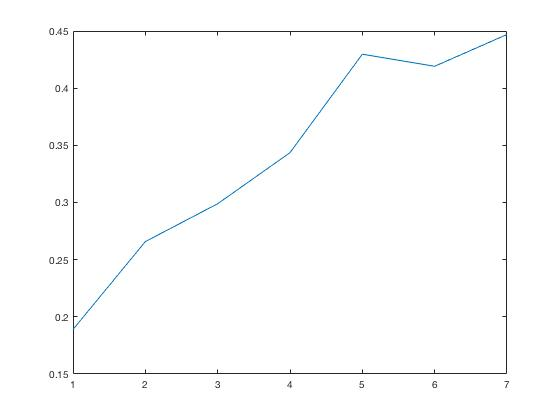
\includegraphics[width=\textwidth]{purity.jpg}
\end{figure}
Horizontal axis represents the $ith$ iteration, for example $3$ is the iteration where $k = 6$.
\newpage{}
\section{Manual calculation of one round of EM for a Mixture of Gaussians}
\subsection{Question 8}
\subsubsection{(a) M Step}
The likelihood is given by $\prod_{i = 1}^{3} \mathbb{P}_{X \sim D_\theta}[X = x_i]$ where each $\mathbb{P}_{X \sim D_\theta}[X = x_i]$ is defined as:
\begin{gather*}
 f_{\theta}(x_i) = \sum_{y = 1}^2 f_\theta(x_i, y)\\
= \sum_{y = 1}^2 \pi_y f_\theta(x_i | y)\\
= \sum_{y = 1}^2 \frac{\pi_y}{\sqrt{2\pi \sigma_{y}^2}} \text{exp}\bigg(-\frac{(x_i - \mu_y)^2}{2 \sigma_{y}^2}\bigg)
\end{gather*}
\subsubsection{(b) M Step}
Computing $N_{y}^{(t)}$:
\begin{gather*}
N_{1}^{(t)} = \sum_{i = 1}^3 Q_{i, 1}^{(t)} = 1 + .4 + 0 = 1.4\\
N_{2}^{(t)} = \sum_{i = 1}^3 Q_{i, 2}^{(t)} = 0 + .6 + 1 = 1.6
\end{gather*}
Computing $\pi_{y}^{(t)}$:
\begin{gather*}
\pi_{1}^{(t)} = \frac{N_1}{3} = \frac{1.4}{3}\\
\pi_{2}^{(t)} = \frac{N_2}{3} = \frac{1.6}{3}
\end{gather*}
\subsubsection{(c) M Step}
Computing $\mu_{y}^{(t)}$:
\begin{gather*}
\mu_{1}^{(t)} = \frac{1}{N_1} \sum_{i = 1}^{m} Q_{i, 1}^{(t)} x_i = \frac{1 + 4 + 0}{1.4} = \frac{5}{1.4}\\
\mu_{2}^{(t)} = \frac{1}{N_2} \sum_{i = 1}^{m} Q_{i, 2}^{(t)} x_i = \frac{0 + 6 + 20}{1.6} = \frac{26}{1.6}
\end{gather*}
\subsubsection{(d) M Step}
Computing $\sigma_{y}^{(t)}$:
\begin{gather*}
\sigma_{1}^{(t)} = \frac{1}{N_1} \sum_{i = 1}^{m} Q_{i, 1}^{(t)} (x_i - \mu_{1})^2 = \frac{(-\frac{3.6}{1.4})^2 + .4 \cdot (\frac{9}{1.4})^2 + 0}{1.4} = \frac{23.14285714}{1.4} = 16.53061224\\
\sigma_{2}^{(t)} = \frac{1}{N_2} \sum_{i = 1}^{m} Q_{i, 2}^{(t)} (x_i - \mu_{2})^2 = \frac{0 + .6 \cdot (-\frac{10}{1.6})^2 + (\frac{6}{1.6})^2}{1.6} = \frac{37.5}{1.6} = 23.4375
\end{gather*}
\subsubsection{(e) E Step}
\begin{gather*}
Q_{i, y}^{(t + 1)} = \frac{\frac{\pi_{y}^{(t)}}{\sigma_{y}^{(t)}} \cdot \text{exp}\bigg(-\frac{(x_i - \mu_{y}^{(t)})^2}{2(\sigma_{y}^{(t)})^2}\bigg)}{\sum_{j = 1}^{k} \frac{\pi_{j}^{(t)}}{\sigma_{j}^{(t)}} \cdot \text{exp}\bigg(-\frac{(x_i - \mu_{j}^{(t)})^2}{2(\sigma_{j}^{(t)})^2}\bigg)}\\
\end{gather*}
Where the value of $y$ is the cluster $c$ which $x_i$ belongs to.
\subsubsection{(f) E Step}
Computing each term in the denominator:
\begin{gather*}
\frac{\pi_{1}^{(t)}}{\sigma_{1}^{(t)}} \cdot \text{exp}\bigg(-\frac{(x_1 - \mu_{1}^{(t)})^2}{2(\sigma_{1}^{(t)})^2}\bigg) = .0282304527 \cdot \text{exp}\bigg( -\frac{6.612244898}{546.5222821} \bigg) = .027890957\\
\frac{\pi_{2}^{(t)}}{\sigma_{2}^{(t)}} \cdot \text{exp}\bigg(-\frac{(x_1 - \mu_{2}^{(t)})^2}{2(\sigma_{2}^{(t)})^2}\bigg) = .0227555556 \cdot \text{exp}\bigg( -\frac{232.5625}{1098.632813} \bigg) = .0184142673\\
\frac{\pi_{1}^{(t)}}{\sigma_{1}^{(t)}} \cdot \text{exp}\bigg(-\frac{(x_2 - \mu_{1}^{(t)})^2}{2(\sigma_{1}^{(t)})^2}\bigg) = .0282304527 \cdot \text{exp}\bigg( -\frac{41.32653061}{546.5222821} \bigg) = .0261744565\\
\frac{\pi_{2}^{(t)}}{\sigma_{2}^{(t)}} \cdot \text{exp}\bigg(-\frac{(x_2 - \mu_{2}^{(t)})^2}{2(\sigma_{2}^{(t)})^2}\bigg) = .0227555556 \cdot \text{exp}\bigg( -\frac{39.0625}{1098.632813} \bigg) = .021960684\\
\frac{\pi_{1}^{(t)}}{\sigma_{1}^{(t)}} \cdot \text{exp}\bigg(-\frac{(x_3 - \mu_{1}^{(t)})^2}{2(\sigma_{1}^{(t)})^2}\bigg) = .0282304527 \cdot \text{exp}\bigg( -\frac{269.8979592}{546.5222821} \bigg) = .017228329\\
\frac{\pi_{2}^{(t)}}{\sigma_{2}^{(t)}} \cdot \text{exp}\bigg(-\frac{(x_3 - \mu_{2}^{(t)})^2}{2(\sigma_{2}^{(t)})^2}\bigg) = .0227555556 \cdot \text{exp}\bigg( -\frac{14.0625}{1098.632813} \bigg) = .0224661407\\
\sum_{j = 1}^{k} \frac{\pi_{j}^{(t)}}{\sigma_{j}^{(t)}} \cdot \text{exp}\bigg(-\frac{(x_1 - \mu_{j}^{(t)})^2}{2(\sigma_{j}^{(t)})^2}\bigg) = .0463052243\\
\sum_{j = 1}^{k} \frac{\pi_{j}^{(t)}}{\sigma_{j}^{(t)}} \cdot \text{exp}\bigg(-\frac{(x_2 - \mu_{j}^{(t)})^2}{2(\sigma_{j}^{(t)})^2}\bigg) = .0481351405\\
\sum_{j = 1}^{k} \frac{\pi_{j}^{(t)}}{\sigma_{j}^{(t)}} \cdot \text{exp}\bigg(-\frac{(x_3 - \mu_{j}^{(t)})^2}{2(\sigma_{j}^{(t)})^2}\bigg) = .0396944697\\
\end{gather*}
Computing $Q_{i, j}^{(t + 1)}$:
\begin{gather*}
Q_{1, 1}^{(t + 1)} = .027890957 / .0463052243 = .6023285152\\
Q_{1, 2}^{(t + 1)} = .0184142673 / .0463052243 = .3976714848\\
Q_{2, 1}^{(t + 1)} = .0261744565 / .0481351405 = .5437702316\\
Q_{2, 2}^{(t + 1)} = .021960684 / .0481351405 = .4562297684\\
Q_{3, 1}^{(t + 1)} = .017228329 / .0396944697 = .4340234075\\
Q_{3, 2}^{(t + 1)} = .0224661407 / .0396944697 = .5659765925
\end{gather*}
Thus \[
   Q^{(t + 1)} =
  \left[ {\begin{array}{cc}
  .6023285152 & .3976714848\\
  .5437702316 & .4562297684\\
  .4340234075 & .5659765925
  \end{array} } \right]
\]

\end{document} 